% Preface required in the knitr RnW file
\documentclass{article}\usepackage[]{graphicx}\usepackage[]{color}
%% maxwidth is the original width if it is less than linewidth
%% otherwise use linewidth (to make sure the graphics do not exceed the margin)
\makeatletter
\def\maxwidth{ %
  \ifdim\Gin@nat@width>\linewidth
    \linewidth
  \else
    \Gin@nat@width
  \fi
}
\makeatother

\definecolor{fgcolor}{rgb}{0.345, 0.345, 0.345}
\newcommand{\hlnum}[1]{\textcolor[rgb]{0.686,0.059,0.569}{#1}}%
\newcommand{\hlstr}[1]{\textcolor[rgb]{0.192,0.494,0.8}{#1}}%
\newcommand{\hlcom}[1]{\textcolor[rgb]{0.678,0.584,0.686}{\textit{#1}}}%
\newcommand{\hlopt}[1]{\textcolor[rgb]{0,0,0}{#1}}%
\newcommand{\hlstd}[1]{\textcolor[rgb]{0.345,0.345,0.345}{#1}}%
\newcommand{\hlkwa}[1]{\textcolor[rgb]{0.161,0.373,0.58}{\textbf{#1}}}%
\newcommand{\hlkwb}[1]{\textcolor[rgb]{0.69,0.353,0.396}{#1}}%
\newcommand{\hlkwc}[1]{\textcolor[rgb]{0.333,0.667,0.333}{#1}}%
\newcommand{\hlkwd}[1]{\textcolor[rgb]{0.737,0.353,0.396}{\textbf{#1}}}%
\let\hlipl\hlkwb

\usepackage{framed}
\makeatletter
\newenvironment{kframe}{%
 \def\at@end@of@kframe{}%
 \ifinner\ifhmode%
  \def\at@end@of@kframe{\end{minipage}}%
  \begin{minipage}{\columnwidth}%
 \fi\fi%
 \def\FrameCommand##1{\hskip\@totalleftmargin \hskip-\fboxsep
 \colorbox{shadecolor}{##1}\hskip-\fboxsep
     % There is no \\@totalrightmargin, so:
     \hskip-\linewidth \hskip-\@totalleftmargin \hskip\columnwidth}%
 \MakeFramed {\advance\hsize-\width
   \@totalleftmargin\z@ \linewidth\hsize
   \@setminipage}}%
 {\par\unskip\endMakeFramed%
 \at@end@of@kframe}
\makeatother

\definecolor{shadecolor}{rgb}{.97, .97, .97}
\definecolor{messagecolor}{rgb}{0, 0, 0}
\definecolor{warningcolor}{rgb}{1, 0, 1}
\definecolor{errorcolor}{rgb}{1, 0, 0}
\newenvironment{knitrout}{}{} % an empty environment to be redefined in TeX

\usepackage{alltt}

\usepackage{rotating}
\usepackage{graphics}
\usepackage{latexsym}
\usepackage{color}
\usepackage{listings} % allows for importing code scripts into the tex file
\usepackage{amsmath}

% Approximately 1 inch borders all around
\setlength\topmargin{-.56in}
\setlength\evensidemargin{0in}
\setlength\oddsidemargin{0in}
\setlength\textwidth{6.49in}
\setlength\textheight{8.6in}

% change name of Abstract
\renewcommand{\abstractname}{Executive Summary}
% allow multiple sections in appendix
\usepackage[title]{appendix}

\title{The Effect of New Housing Projects on Expenditures in Two New York Municipalities} 
\author{Andrew Bates}
\date{October 11, 2018}
\IfFileExists{upquote.sty}{\usepackage{upquote}}{}
\begin{document} 
\maketitle

\begin{abstract}
In this paper we estimate future expenditures for two municipalites in New York based on various projected demographic and income-related factors. These estimates are obtained from a linear model chosen via a stepwise regression procedure with AIC as the model selection criterion. The variables in the model are wealth per person, population, percent intergovernmental funding, and growth rate. The estimated expenditures for Warwick are 1, 2 for the years 2005 and 2025. The estimated expenditures for Monroe are 1, 2 for the years 2005 and 2025.
\end{abstract}


\section{Introduction} \label{intro}

Two New York towns, Warwick and Monroe, would like to estimate future expenditures triggered by new housing construction proposals. They are primarily interested in determining whether they need to increase funds to compensate for increased expenditures related to the housing projects. To construct these estimates, Warwick and Monroe obtained data on expenditures along with various demographic and income-related variables from several New York municiplaties. 

\section{Methods} \label{methods}

The data used in this study consisted of 916 observations of seven variables. Each observation corresponds to a New York municipality for which each of the variables were collected. The response variable is expenditure per person. The covariates are as follows: wealth per person, population, revenue from state and federal grants, population density, mean income per person, and growth rate.

For reasons of simplicity and interpretability, a linear regression model was chosen to estimate future expenditures. The correlation between population and population density was high ($0.67$) so to prevent this from leading to multicolinearity issues, only population was considered in the analysis. The variables in this data set (including the response) were heavily skewed, so log transformations were applied to each. To ensure a linear relationship between the predictors and the response, the data was subsetted to include only those observations for which the population was larger than $4,000$. The projected covariates for Warwick and Monroe fall within the range of the covariates in the subsetted data so we felt this method was appropriate. In addition, this method was favored over a more complicated method like including a quadratic term on log population which would be harder to interpret. The regression model was constructed via stepwise regression using AIC as the selection criterion. This model was then used to estimate future expenditures.



\section{Analysis} \label{analysis}




\subsection{Exploratory Data Analysis} \label{eda}

In this data set there were two measures of the size of a municipality: population and population density. Unsurprisingly, the correlation between these two measures was relatively high ($0.67$). In the interest of parsimony and to mitigate possible colinearity issues, we decided to consider only one of these variables to construct our model. Population density had a moderate correlation with mean income per person ($0.49$) whereas population had a comparably low correlation with income ($0.29$). To hedge against problems with colinearity, we decided to consider population for the model building process.

Upon an initial examination of the data, it was evident that transformations would be necessary. Each of the covariates, and the response, were skewed (see Appendix \ref{appendix_plots}) and some were heavily skewed. As this might pose problems with linearity, we performed transformations on the variables. To remain in line with our goal of having a comprehensible model, we favored log transformations over a more complex procedure. To that end, we performed log transformations on all variables in the data set.  However, a straightforward application of the logarithm was not possible for one covariate. Growth rate contains some negative values as well as some zero values. To remedy this, we used the following pseudo-log transformation:
\[
\text{p-}\log(\text{growth rate}) = % plog for pseudo-log
  \begin{cases}
    \log(\text{growth rate} + 0.15) &\text{if growth rate} > 0 \\
    -\log(-\text{growth rate} + 0.15) &\text{if growth rate} \le 0.
  \end{cases}
\]
Note that since this is a one-to-one transformation ...

To ensure the linearity assumption of our model was satisfied, we examined the relationship between log expenditure and the log of each of the covariates. Except for log population, all other covariates had an approximately liner relationship with log expenditure. Figure \ref{fig:vs_log_pop} is a plot of log expenditure vs. log population with the addition of a smoothing line. We see what appears to be a quadratic relationship. However, notice that on either side of the vertical line (corresponding to a log population of $8.3$), the relationship is approximately linear. So we were essentially faced with two choices. We could try to include the square of log population as an additional predictor or we could subset the data and have a roughly linear relationship between the response and log population.


\begin{knitrout}
\definecolor{shadecolor}{rgb}{0.969, 0.969, 0.969}\color{fgcolor}\begin{figure}[h]
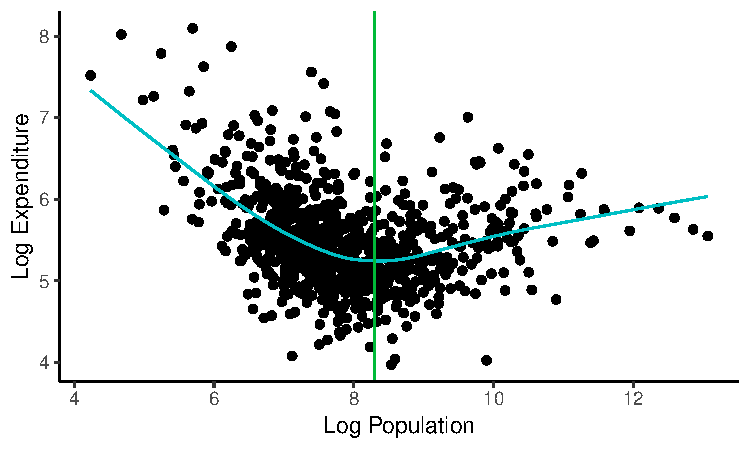
\includegraphics[width=\maxwidth]{figure/r_fig_vs_log_pop-1} \caption{\label{fig:vs_log_pop} Plot of log expenditure vs. log population with LOWESS smooth line}\label{fig:r fig_vs_log_pop}
\end{figure}


\end{knitrout}

We chose the latter method. As mentioned previously, we favored a simpler model for the interpretability that comes with it. The log of population squared is not as easy to understand. Also, the projected covariates we would be predicting with fall within the rang of the covariates in the subsetted data. For these reasons, we subsetted the data to include only those observations that had a population greater than $4,000$ (log population above $8.3$). This subsetted data set included $266$ of the original observations which we felt was large enough to obtain accurate inferences from. Figure \ref{fig:vs_log_pop_subset} is a plot of log expenditure vs. log population for this subsetted data set along with a smoothing line. We can see that the relationship between the two variables is roughly linear. We do see minor deviation from linearity for high values of log population but overall the trend is approximately linear. Additionally, it is much more linear than the relationship we see in Figure \ref{fig:vs_log_pop}.

\begin{knitrout}
\definecolor{shadecolor}{rgb}{0.969, 0.969, 0.969}\color{fgcolor}\begin{figure}[h]
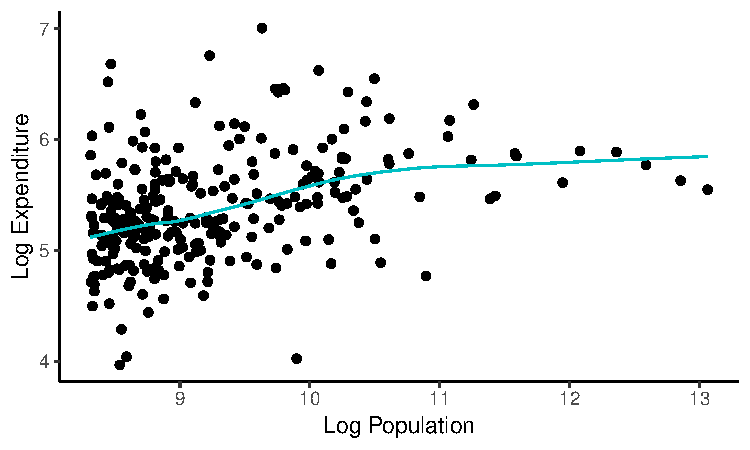
\includegraphics[width=\maxwidth]{figure/r_fig_vs_log_pop_subset-1} \caption{\label{fig:vs_log_pop_subset} Plot of log expenditure vs. log population with LOWESS smooth line from subsetted data}\label{fig:r fig_vs_log_pop_subset}
\end{figure}


\end{knitrout}

\subsection{Modeling and Diagnostics} \label{modeling}

After performing variable transformations and data subsetting, our regression model was ready to be constructed. We used both forward and backward stepwise regression to build the model. AIC was used as our model selection criterion. This was partly due to the ubiquity of AIC and partly because it penalizes larger models. This penalization aligns itself with our preference for simpler models. That being said, we did investigate the inclusion of squared log transformations for all the covariates ($\log^2(\text{income})$, etc.). However, there was not much of an improvement that could be gained by including these terms. The AIC for the model including these terms was $-622$ while the AIC for the model without them was $-611$, not much of a difference. Furthermore, the model with the quadratic variables included contained some quadratic terms without their corresponding linear components. We simply could not justify such a model.

The final model used log expenditure as the response with the following covariates: log wealth, log population, log percent intergovernmental funding, and log growth rate.

From here: 

a bit more about the model like mentioning p-values and VIF's. include table with regression summary. analyze the table. i.e. log grow rate has a very small coefficient (-0.02). explain why this may or may not be useful (think effect size). reference to Table \ref{tbl:regress}


% latex table generated in R 3.5.1 by xtable 1.8-3 package
% Tue Oct  9 09:22:22 2018
\begin{table}[ht]
\centering
\begin{tabular}{|l|rrrr|}
  \hline
 & Estimate & SE & p-value & 95\% CI \\ 
  \hline
Intercept & 0.13 & 0.44 & 0.769 & ( -0.73 , 0.99 ) \\ 
  Log Wealth & 0.49 & 0.04 & 0.000 & ( 0.42 , 0.56 ) \\ 
  Log Population & 0.08 & 0.02 & 0.001 & ( 0.03 , 0.12 ) \\ 
  Log \% Intergov Funding & -0.28 & 0.04 & 0.000 & ( -0.36 , -0.20 ) \\ 
  Log Growth Rate & -0.02 & 0.01 & 0.031 & ( -0.05 , -0.00 ) \\ 
   \hline
\end{tabular}
\caption{Summary table for regressing log expenditure on 
         log wealth, log population, log percent government funding,
         and log growth rate} 
\label{tbl:regress}
\end{table}




include diagnostic plots. residual vs. fitted. either qq plot or histogram of residuals (note the outlier or 2 on the left of this plot). may want to consider other residuals like studentized. may also want to consider having this come before the tables. not sure the best order here.

make predictions. give table with projected wealth, income, etc. then give table of predictions with PI's. be sure to try to find anything interesting to talk about. this might go in a 'Results' section

\section{Conclusion} \label{conclusion}



\newpage
\begin{appendices}

\section{Supplementary Plots} \label{appendix_plots}

\end{appendices}


\end{document}
